\subsubsection{PML Parameters}

Having validated the solver against benchmark CAA solutions, the controlling parameters may now be explored for their effect on the accuracy of the solutions. Parameters under investigation are those outlined earlier in Section \ref{PerfectlyMatchedLayerMethodSection}, summarised as the damping profile $
\Gamma$, damping coefficient $\sigma$, and PML width $D$. Ultimately, the PML is a non-reflective BC but only under certain parameterised circumstances, and can easily be setup where spurious waves and errors are supported. Thus, the parameters should be configured to meet this non-reflectivity, but importantly to also keep the domain small and efficient with ideally the smallest PML width possible.

To standardise the parameter optimisation process, the initial conditions described in Equation \ref{eq:BenchmarkEqs} are used with some slight modifications: the density condition is modified to remove the $0.1 e^{\left[ - \left( \mathrm{ln} \, 2 \right) \\ \left( \left(x-x_2 \right)^2 + \left(y-y_2 \right)^2 \right)/25 \right]}$ term, the location of the pulses are set to $\left(0,0\right)$, and the mean flow is removed (for reasons which will become clear). The error calculation used to compare parameters in this section uses the pressure variable, comparing the inner domain of both the standard and reference domain (outlined in Section \ref{GridSection}).


The damping profile as defined by Equation \ref{PMLProfileEq} controls the distribution of the damping throughout the PML layer according to a power law, and has the least degrees of freedom out of the PML parameters. It will therefore be explored first to find a suitable power and reduce the parameterisation later in the investigation.

Using an unoptimised configuration of $D_{x,y}=30\Delta x$ and $\sigma_{x,y}=2$, the powers from 1 through 4 (linear to quartic) are assessed for reflection error when subject to a simple Gaussian pulse. Figure \ref{fig:VariedProfile} illustrates the variation in distribution for the varying powers, and Figure \ref{fig:PMLProfile} shows the reflection error of each power over a 2.5 second simulation.


\begin{figure}[h!]
    \centering
    \begin{subfigure}[h]{0.45\textwidth}
        \centering
        \makebox[0pt]{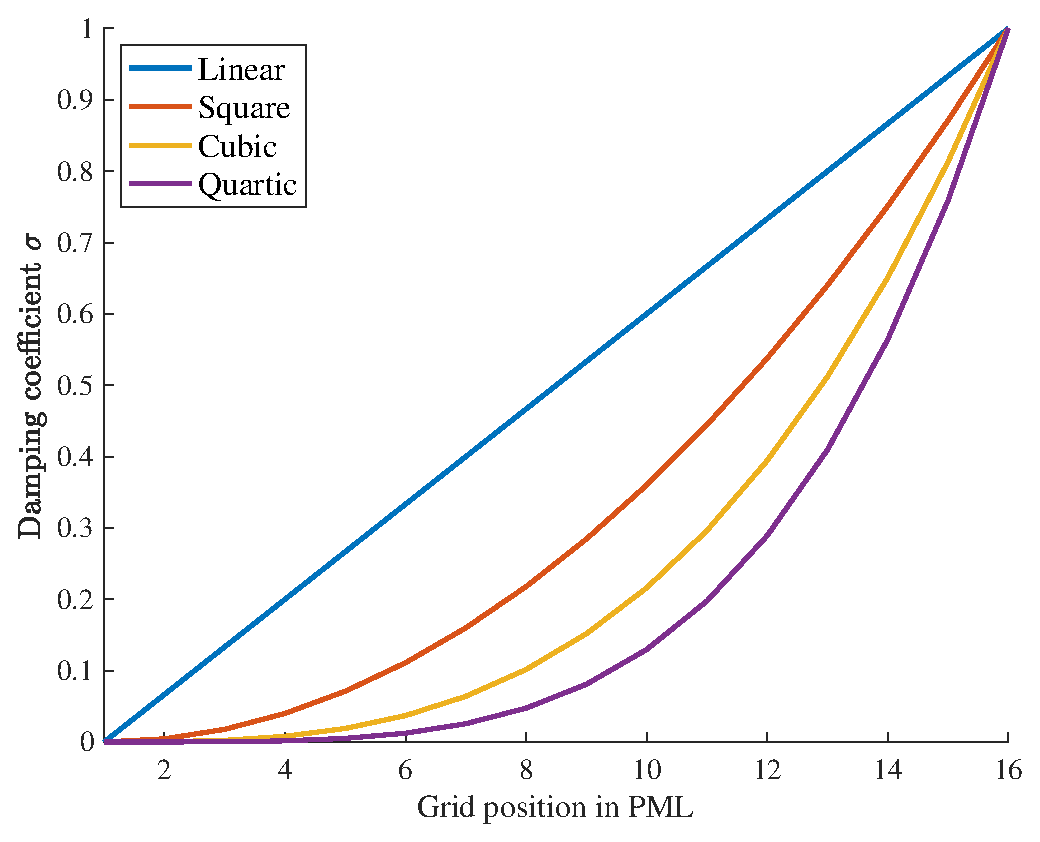
\includegraphics[width=7cm]{Figures/TechnicalAchievement/Res/variedProfile.eps}}
        \caption{}
        \label{fig:VariedProfile}
    \end{subfigure}
    \hfill
    \begin{subfigure}[h]{0.49\textwidth}
        \centering
        \makebox[0pt]{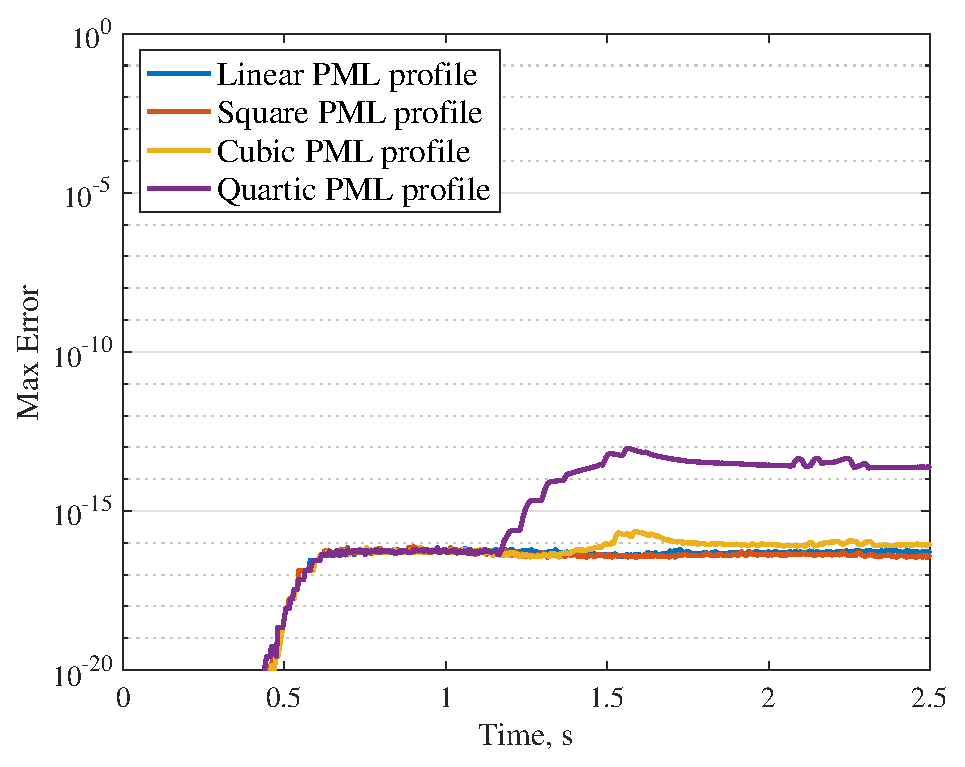
\includegraphics[width=7cm]{Figures/TechnicalAchievement/Res/PMLProfiles.eps}}
        \caption{}
        \label{fig:PMLProfile}
    \end{subfigure}
    \caption{\textbf{(a)} Variation in the damping distribution within the PML layer using differing powers. \textbf{(b)} Max reflection error of differing power profiles using standard, unoptimised parameters of $D=30\Delta x$ and $\sigma_{x,y}=2$.
    }
    \label{fig:PMLDistribution}
\end{figure}

\newpage

Evidently the quartic profile incurs significantly higher reflectivity than the other profiles. This is likely as it takes longer to ramp up the damping coefficient and produces a much sharper change in damping towards the last third of the PML layer - causing the decay rate to be too drastic and not allowing for smooth absorption within the spatial discretisation scheme. The cubic profile also exhibits some minor error but is similar in stability to the lower powers. The square profile offers the greatest medium between gently increasing the damping and avoiding sharp jumps at the Euler/PML boundary (as the linear profile shows) - thus it is selected as a static parameter for the remainder of the results.


The investigation of damping coefficient effects following similarly from the profile, however, given it's importance in PML performance it seems prudent to demonstrate the effects via contour plots. The effects of varying the damping coefficient are noticeably indistinguishable when comparing entire simulations of differing parameters. Thus, a quarter section of the domain for each damping coefficient has been combined (the initial condition is centered in the domain with no mean flow) for each timestep - to intuitively compare the effects. Results of simulations with damping coefficients $\sigma_{x,y}=0.5, 1, 1.5, 2$ are shown below in Figure \ref{fig:Damping}.


\begin{figure}[h!]
        \centering
        \begin{subfigure}[b]{0.475\textwidth}
            \centering
            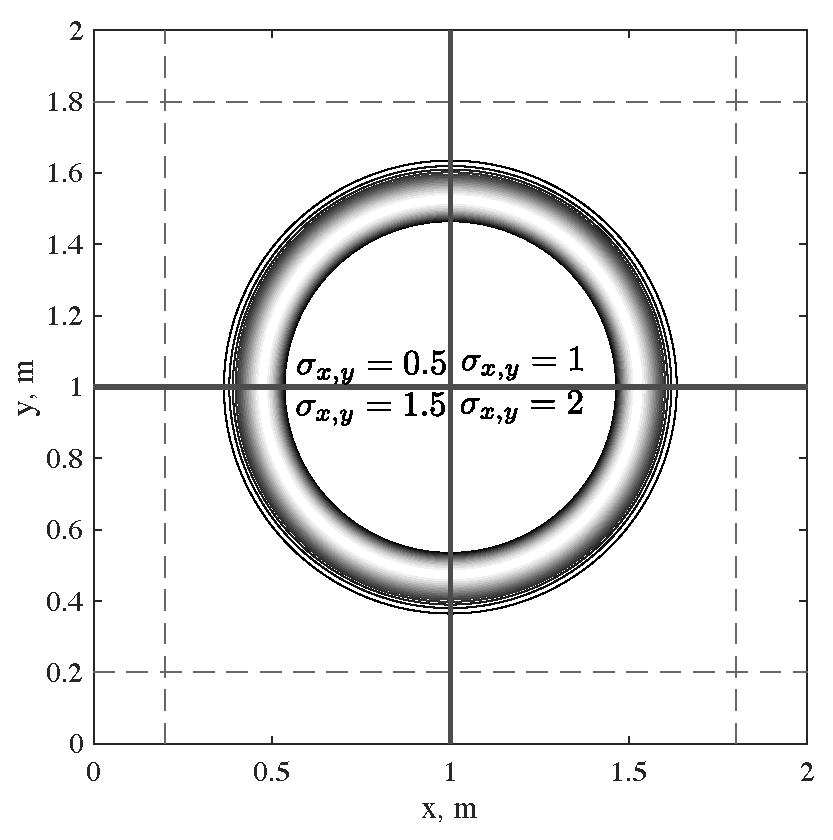
\includegraphics[width=7cm]{Figures/TechnicalAchievement/Res/Damping05s.eps}
            \caption{}    
            \label{fig:Damping05}
        \end{subfigure}
        \hfill
        \begin{subfigure}[b]{0.475\textwidth}  
            \centering 
            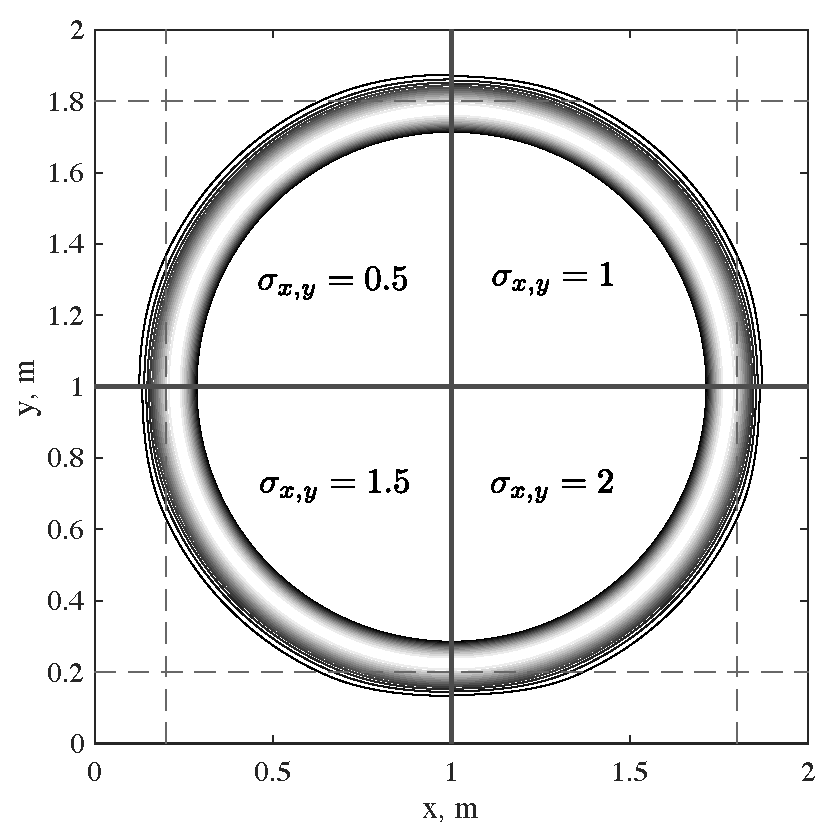
\includegraphics[width=7cm]{Figures/TechnicalAchievement/Res/Damping075s.eps}
            \caption{}  
            \label{fig:Damping075}
        \end{subfigure}
        \vskip\baselineskip
        \vspace{-0.5cm}
        \begin{subfigure}[b]{0.475\textwidth}   
            \centering 
            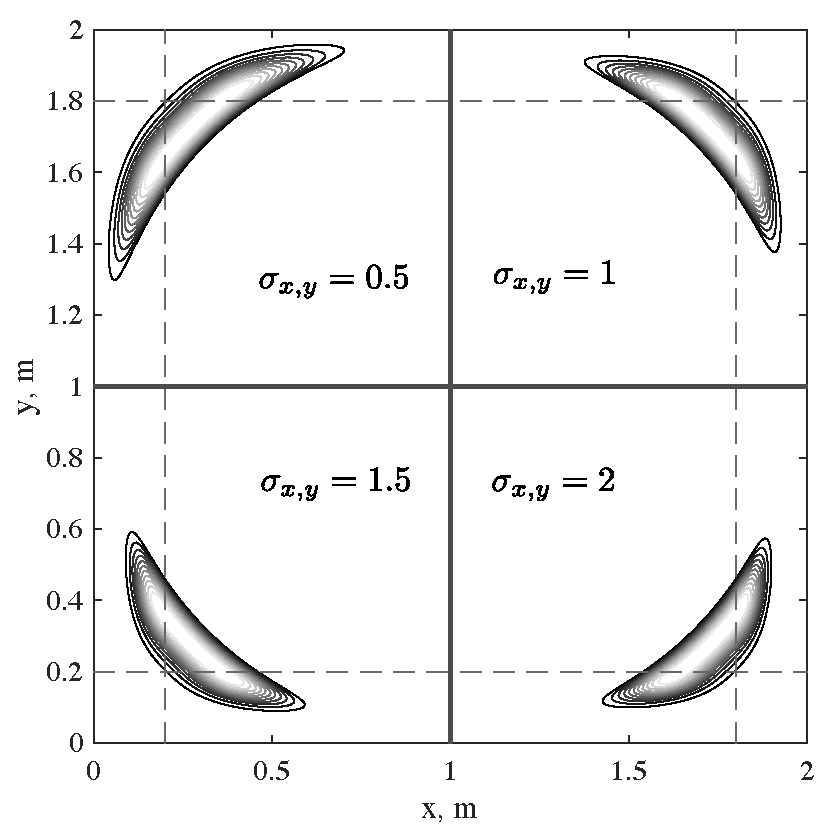
\includegraphics[width=7cm]{Figures/TechnicalAchievement/Res/Damping1s.eps}
            \caption{}  
            \label{fig:Damping1}
        \end{subfigure}
        \hfill
        \begin{subfigure}[b]{0.475\textwidth}   
            \centering 
            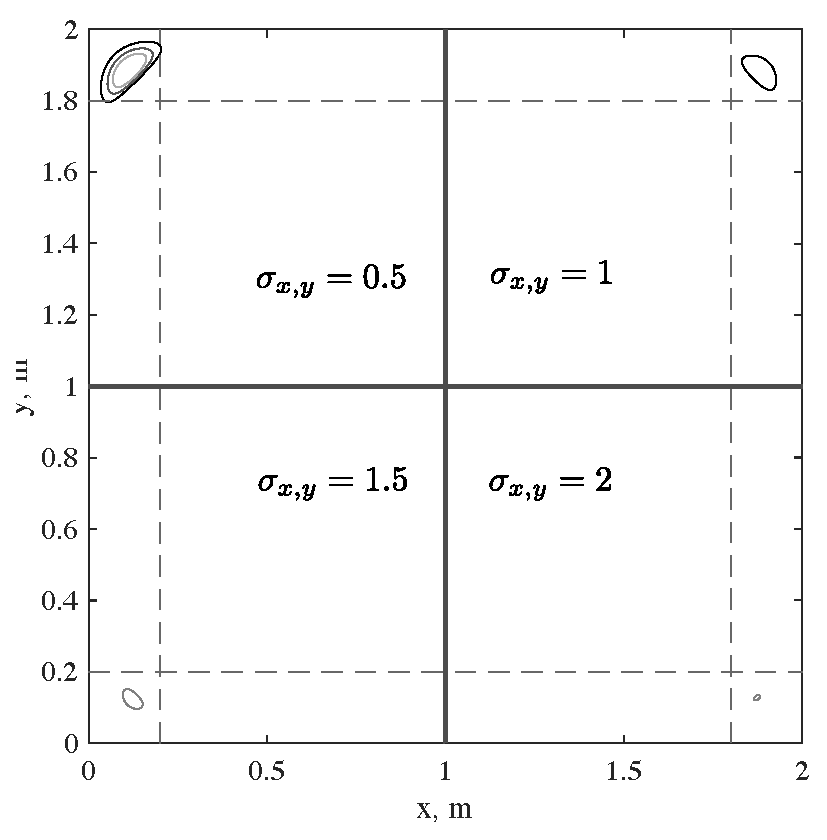
\includegraphics[width=7cm]{Figures/TechnicalAchievement/Res/Damping125s.eps}
            \caption{} 
            \label{fig:Damping125}
        \end{subfigure}
        \caption{Density contours ranging from $\pm0.005$ to $\pm0.1$, showing an acoustical pulse with PML damping coefficients of $\sigma_{x,y}=0.5,1,1.5,2$ at snapshot times. Freestream Mach number set to $M=0$, with $D_{x,y}=30 \Delta x$. \textbf{(a)} $t=0.5 \ \mathrm{s}$, \textbf{(b)} $t=0.75 \ \mathrm{s}$, \textbf{(c)} $t=1 \ \mathrm{s}$, \textbf{(d)} $t=1.25 \ \mathrm{s}$. N.B. Dashed lines indicate PML zones.}
        \label{fig:Damping}
\end{figure}

The effects on the damping of the wave are seen positively within the PML zones, but the induced error in the Euler domain is not as visible (shown later in Figure \ref{fig:DampingError}). Given the relationship between damping coefficient and PML width, it is unwise to draw strong conclusions without assessing them simultaneously - as will be done later in the results.

\clearpage

Next the PML width is varied with $D_{x,y} = 5, 15, 25, 35 \Delta x$ and the effects similarly captured by quarter plots over 4 temporal snapshots (Figure \ref{fig:Width}).


\begin{figure}[h!]
        \centering
        \begin{subfigure}[b]{0.475\textwidth}
            \centering
            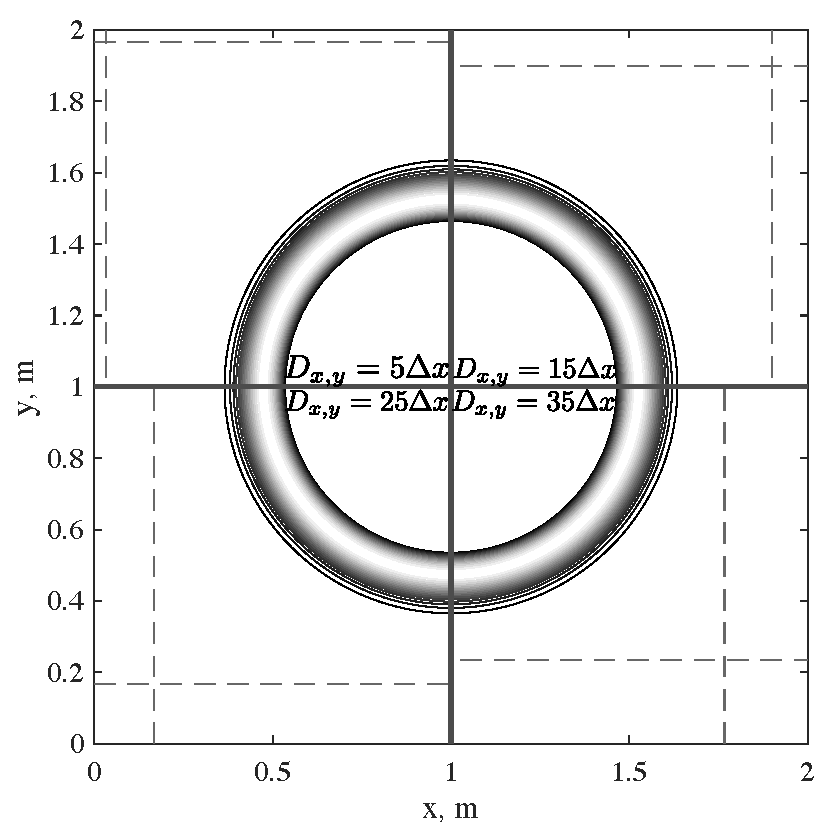
\includegraphics[width=7cm]{Figures/TechnicalAchievement/Res/Width05s.eps}
            \caption{}    
            \label{fig:Width05}
        \end{subfigure}
        \hfill
        \begin{subfigure}[b]{0.475\textwidth}  
            \centering 
            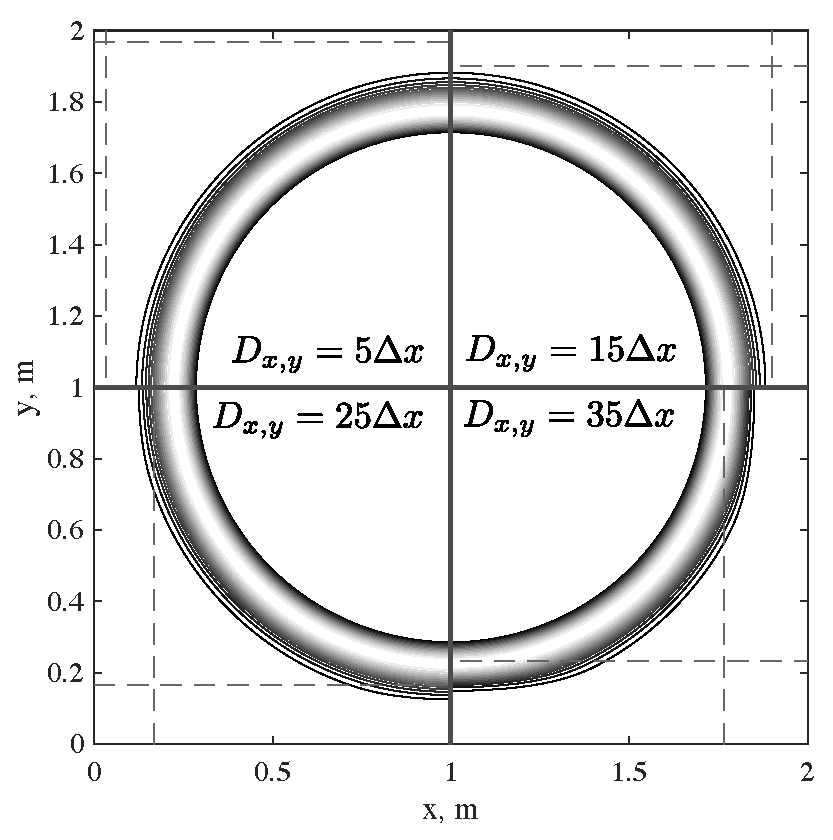
\includegraphics[width=7cm]{Figures/TechnicalAchievement/Res/Width075s.eps}
            \caption{}  
            \label{fig:Width075}
        \end{subfigure}
        \vskip\baselineskip
        \vspace{-0.5cm}
        \begin{subfigure}[b]{0.475\textwidth}   
            \centering 
            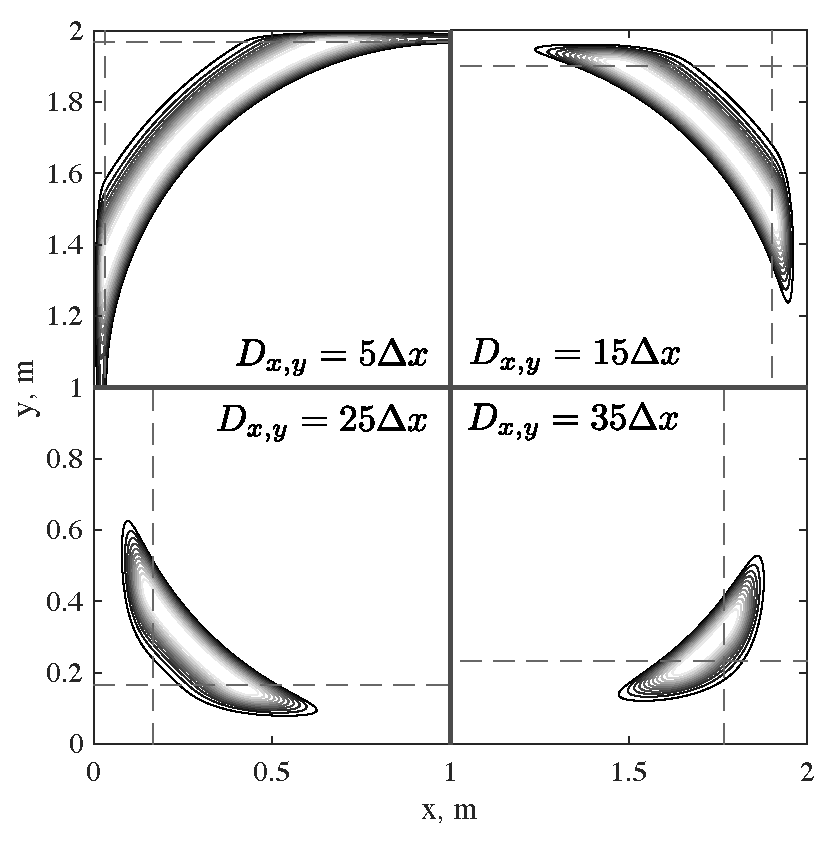
\includegraphics[width=7cm]{Figures/TechnicalAchievement/Res/Width1s.eps}
            \caption{}  
            \label{fig:Width1}
        \end{subfigure}
        \hfill
        \begin{subfigure}[b]{0.475\textwidth}   
            \centering 
            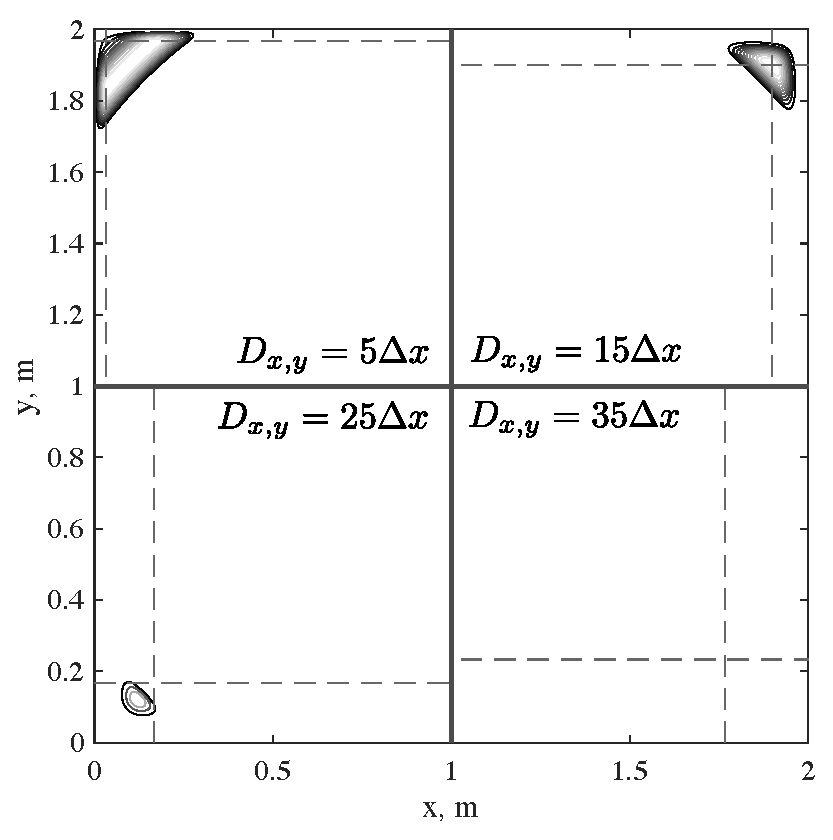
\includegraphics[width=7cm]{Figures/TechnicalAchievement/Res/Width125s.eps}
            \caption{} 
            \label{fig:Width125}
        \end{subfigure}
        \caption{Density contours at ranging from $\pm0.005$ to $\pm0.1$, showing an acoustical pulse with PML widths of $D_{x,y}=5,15,25,35 \Delta x$ at snapshot times. Freestream Mach number set to $M=0$, with $\sigma_{x,y}=2$. \textbf{(a)} $t=0.5 \ \mathrm{s}$, \textbf{(b)} $t=0.75 \ \mathrm{s}$, \textbf{(c)} $t=1 \ \mathrm{s}$, \textbf{(d)} $t=1.25 \ \mathrm{s}$. N.B. Dashed lines indicate PML zones.}
        \label{fig:Width}
\end{figure}

Here, the effects on damping are far easier to see as the smaller PML widths have less grid points to smoothly damp the outgoing waves - which results in compromised wave fronts within the domain thus skewing any phenomena of interest.


Next the induced error of the varying damping coefficients and PML width is assessed as a function of time in Figures \ref{fig:DampingError} and \ref{fig:WidthError}, noting the log scale for the error ranging from $10^{-20}$ to $1$. A line plot along $y=0 \ \mathrm{m}$ also provides another dimension on top of the contour plots, shown for both varying damping coefficients and PML widths in Figures \ref{fig:DampingLinePlot} and \ref{fig:WidthLinePlot}.


\begin{figure}[h]
    \centering
    \begin{subfigure}[h]{0.47\textwidth}
        \centering
        \makebox[0pt]{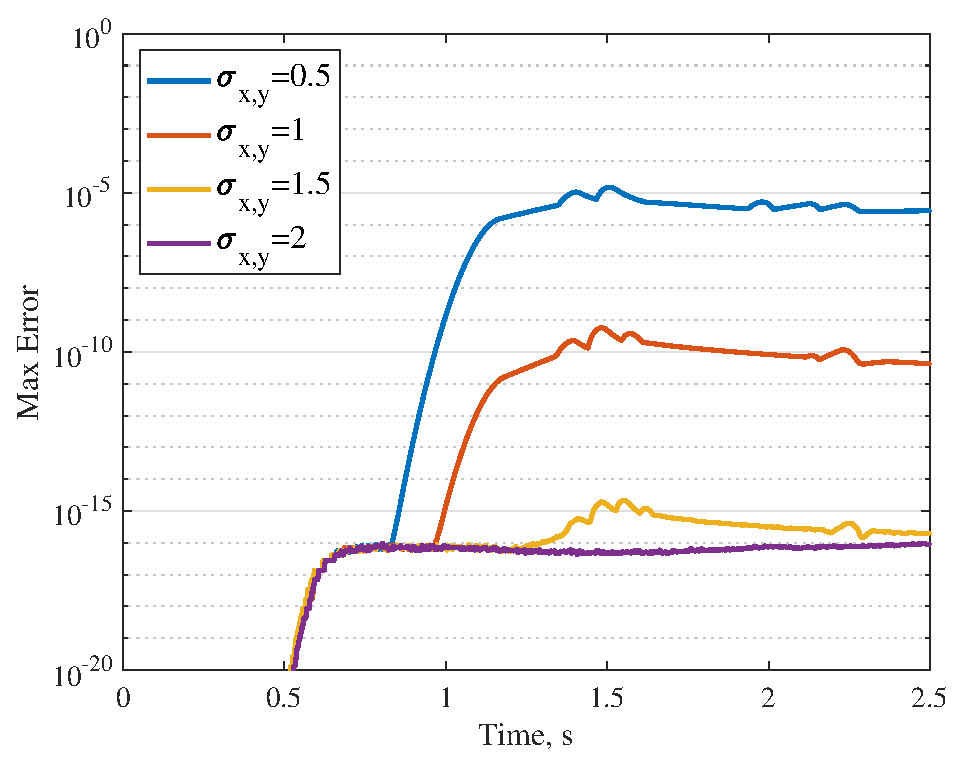
\includegraphics[width=7.5cm]{Figures/TechnicalAchievement/Res/VariedSigma.eps}}
        \caption{}
        \label{fig:DampingError}
    \end{subfigure}
    \hfill
    \begin{subfigure}[h]{0.47\textwidth}
        \centering
        \makebox[0pt]{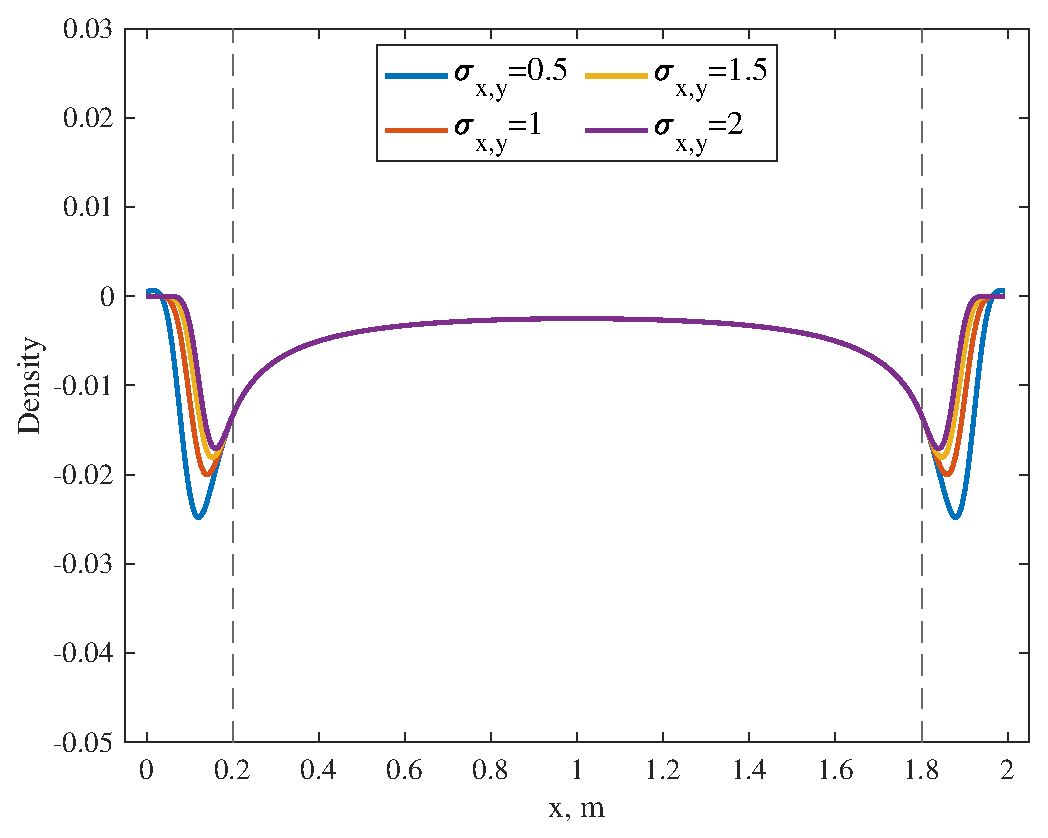
\includegraphics[width=7.5cm]{Figures/TechnicalAchievement/Res/VariedSigmaLine.eps}}
        \caption{}
        \label{fig:DampingLinePlot}
    \end{subfigure}
    \caption{\textbf{(a)} Max Euler domain error of varying damping coefficients for $D_{x,y}=30 \Delta x$ over a $T=2.5 \ \mathrm{s}$ run. \textbf{(b)} Density line plot at $t=0.8 \ \mathrm{s}$, $y=0 \ \mathrm{m}$ showing varying wave decay from differing damping coefficients.}
    \label{fig:DampingAccessories}
\end{figure}


\begin{figure}[h!]
    \centering
    \begin{subfigure}[h]{0.47\textwidth}
        \centering
        \makebox[0pt]{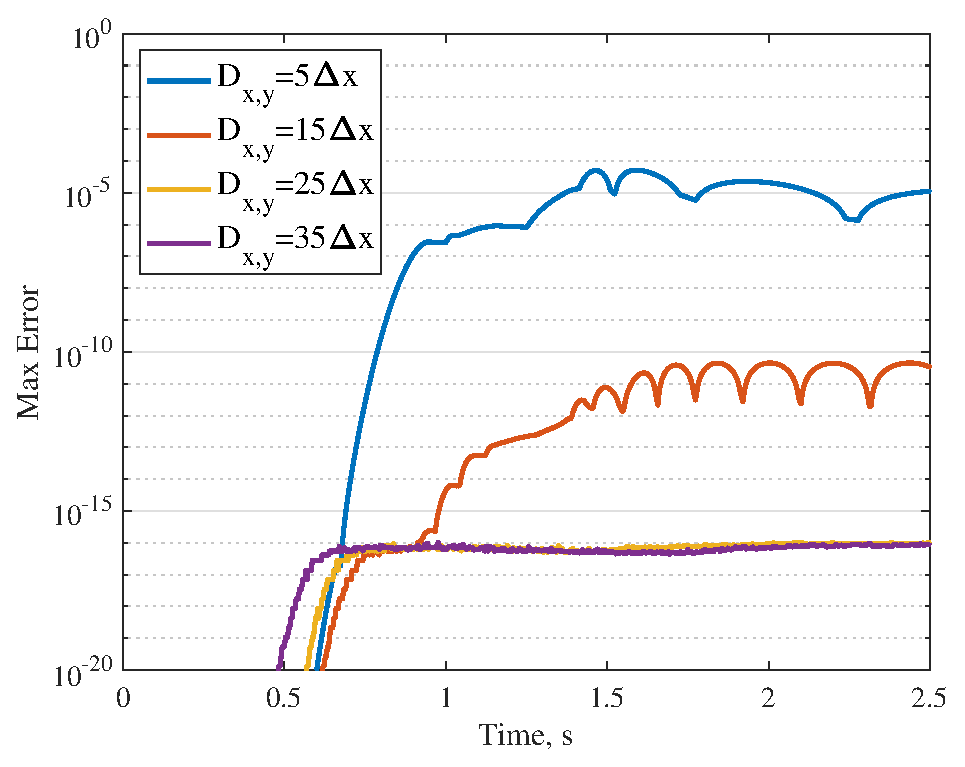
\includegraphics[width=7.5cm]{Figures/TechnicalAchievement/Res/VariedWidth.eps}}
        \caption{}
        \label{fig:WidthError}
    \end{subfigure}
    \hfill
    \begin{subfigure}[h]{0.47\textwidth}
        \centering
        \makebox[0pt]{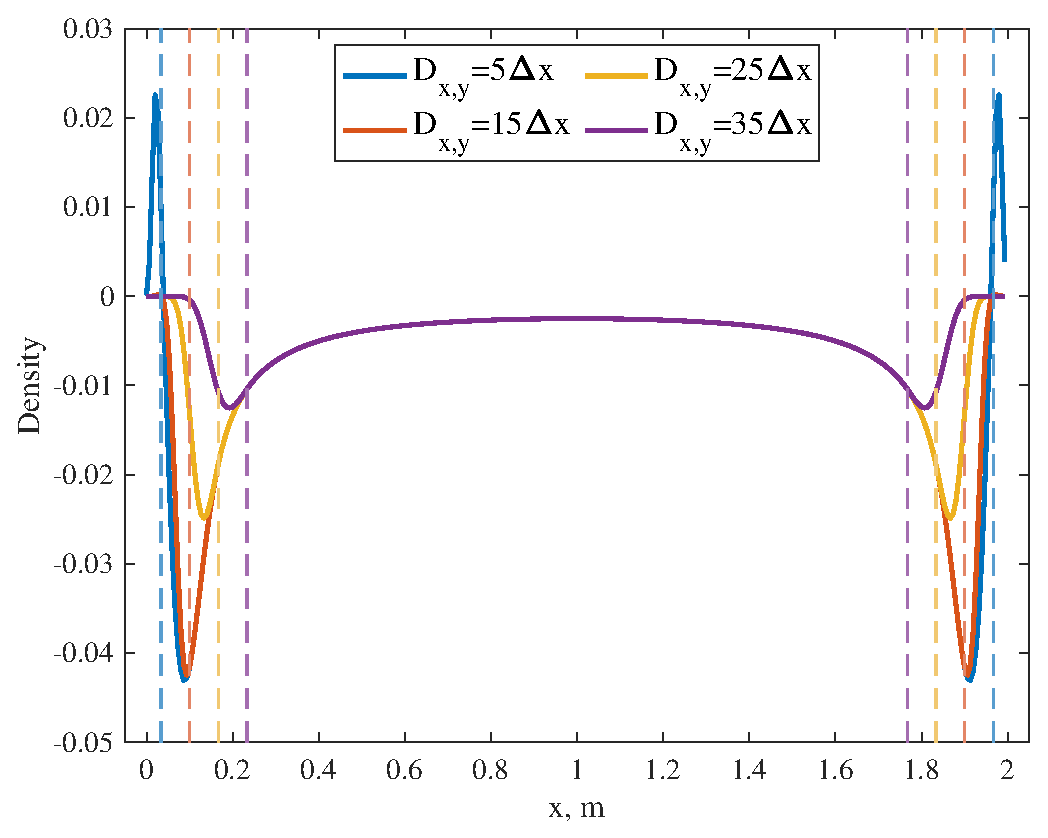
\includegraphics[width=7.5cm]{Figures/TechnicalAchievement/Res/VariedWidthLine.eps}}
        \caption{}
        \label{fig:WidthLinePlot}
    \end{subfigure}
    \caption{\textbf{(a)} Max Euler domain error of varying PML widths for $\sigma_{x,y}=2$ over a $T=2.5 \ \mathrm{s}$ run. \textbf{(b)} Density line plot at $t=0.8 \ \mathrm{s}$, $y=0 \ \mathrm{m}$ showing varying wave decay from differing PML widths.}
    \label{fig:WidthAccessories}
\end{figure}

\newpage

Where it might not have been obvious in the contour plots how much error is induced, the first error plot shows that for a width of $D_{x,y}=30 \Delta x$, damping coefficients below $\sigma_{x,y}=2$ (likely lower but not shown due to granularity of chosen values) are unable to effectively damp the outgoing waves and prevent spurious waves from entering the Euler domain. Then, the second error plot shows that for a coefficient of $\sigma_{x,y}=2$, widths below $D_{x,y}=25 \Delta x$ (again, likely lower) the outgoing waves are not adequately damped before the outer boundary and produce spurious oscillatory motion within the Euler domain.


Ultimately it is a balance between grid width and damping coefficient, and the two cannot be considered exclusively. To explore an optimal range for both parameters, simulations are run with a high number of combinations to determine an effective operating zone. Figure \ref{fig:2DContourSigmaD} shows the maximum error produced in simulations for given $D$ and $\sigma$ combinations, where the bold red line indicates the favourable combinations for reduced error (smallest width for any given damping coefficient). For intuition, Figure \ref{fig:SurfaceSigmaD} shows the operating 'bucket' and demonstrates how the error quickly increases for certain combinations. 



\begin{figure}[h]
    \centering
    \begin{subfigure}[h]{0.49\textwidth}
        \centering
        \makebox[0pt]{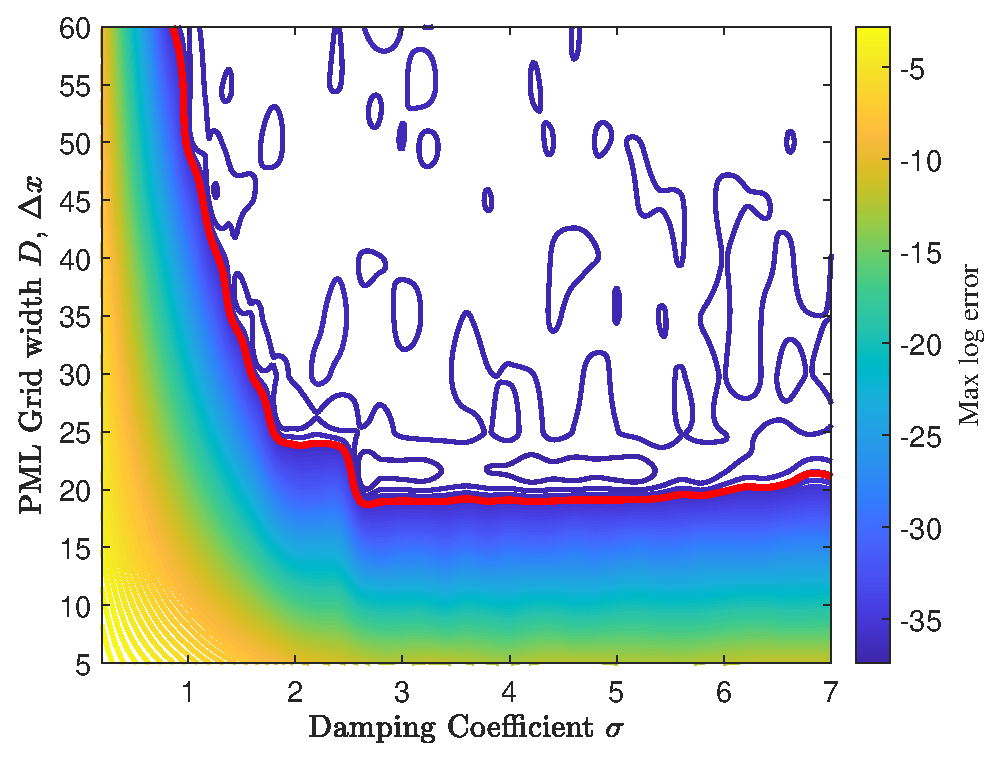
\includegraphics[width=8.5cm]{Figures/TechnicalAchievement/Res/2dContourSigmaD.eps}}
        \caption{}
        \label{fig:2DContourSigmaD}
    \end{subfigure}
    \hfill
    \begin{subfigure}[h]{0.45\textwidth}
        \centering
        \makebox[0pt]{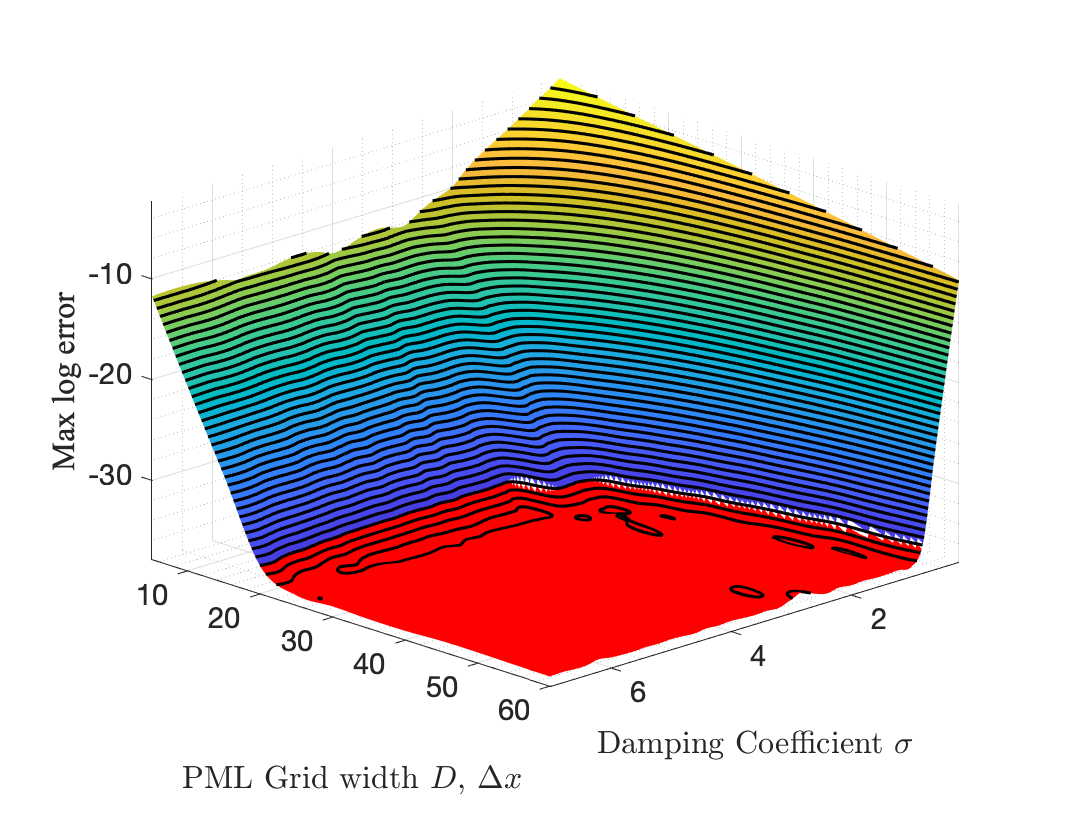
\includegraphics[width=8.5cm]{Figures/TechnicalAchievement/Res/SurfaceSigmaD.eps}}
        \caption{}
        \label{fig:SurfaceSigmaD}
    \end{subfigure}
    \caption{Numerically derived maximum log error (arbitrary units, lower=better) for varying combinations of PML grid width $D$ and damping coefficient $\sigma$. \textbf{(a)} 2d shaded contours and \textbf{(b)} surface plot. N.B red contour line in \textbf{(a)} and red plane in \textbf{(b)} indicate optimal operating region of low error.}
    \label{fig:SigmaDFinal}
\end{figure}

The second goal (after increasing accuracy/reducing error) is to reduce computational effort, which can be taken as reducing the required domain size. Thus, one aims for the smallest stable grid width, which is extracted as $D_{x,y}=19 \Delta x$ with a damping coefficient in the range $2.7 \leq \sigma_{x,y} \leq 5.3$. Interestingly, the results infer that there is no real change in Euler domain error from $\sigma_{x,y}=2.7$ to $\sigma_{x,y}=5.3$. As has been shown in \cite{choung2018nonreflective} (discussed in Section \ref{OptimumCondSection}), spurious waves are invariably observed in over-damped simulations (e.g. $\sigma > 2$). However, the same cannot be stated for the linear solver developed for this project. One might then draw recommendations that a similar CAA solver should use a grid width $D_{x,y}=19 \Delta x$ for a damping coefficient in the range of $2.7 \leq \sigma_{x,y} \leq 5.3$ to maximise computational efficiency whilst maintaining numerical accuracy. But this conclusion conflicts with what has been mathematically derived in \cite{choung2018nonreflective}, and will required further investigation.



As a side note, it might be interesting to see what happens with PML zones of differing widths - as one might encounter with certain geometries. A simulation is run with the benchmark initial conditions, using $D_x=10\Delta x$ and $D_y=40\Delta x$, and subsequently shown in Figure \ref{fig:ncError}. The distribution of error is then shown in Figure \ref{fig:ncErrorDistr}, which indicates the PML $x-$layer provides the majority error (spurious waves propagating parallel with the $y-$layer) as it cannot sufficiently damp the outgoing waves. 

\begin{figure}[h]
    \centering
    \begin{subfigure}[h]{0.45\textwidth}
        \centering
        \makebox[0pt]{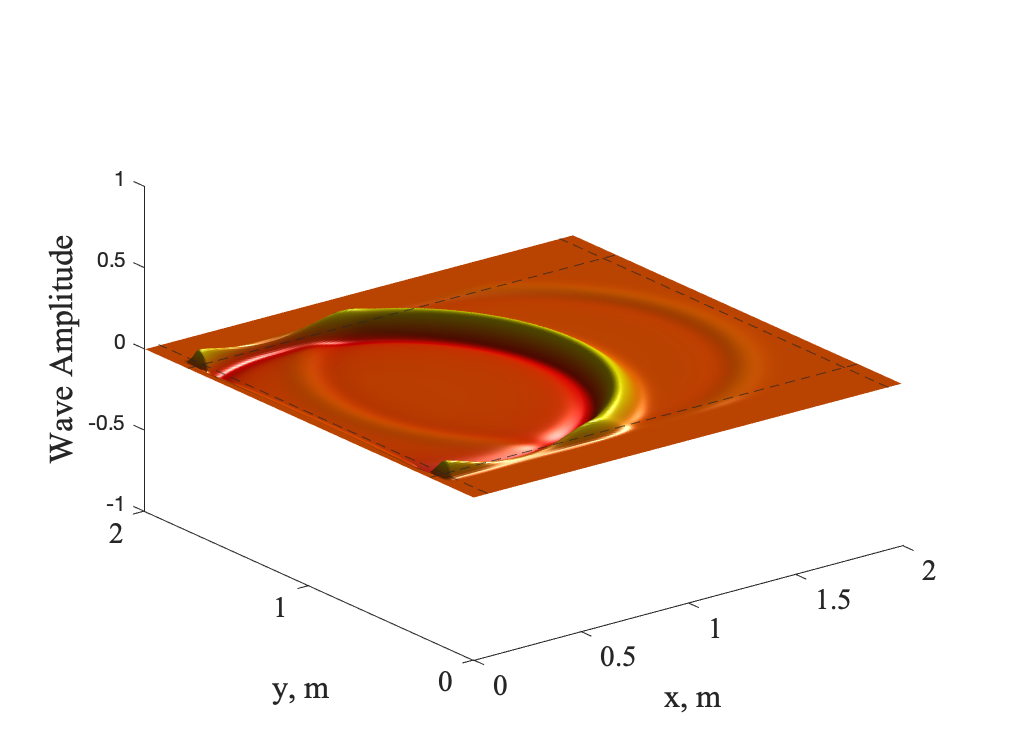
\includegraphics[width=8.5cm]{Figures/TechnicalAchievement/Res/ncSurfAt08s.eps}}
        \caption{}
        \label{fig:ncError}
    \end{subfigure}
    \hfill
    \begin{subfigure}[h]{0.45\textwidth}
        \centering
        \makebox[0pt]{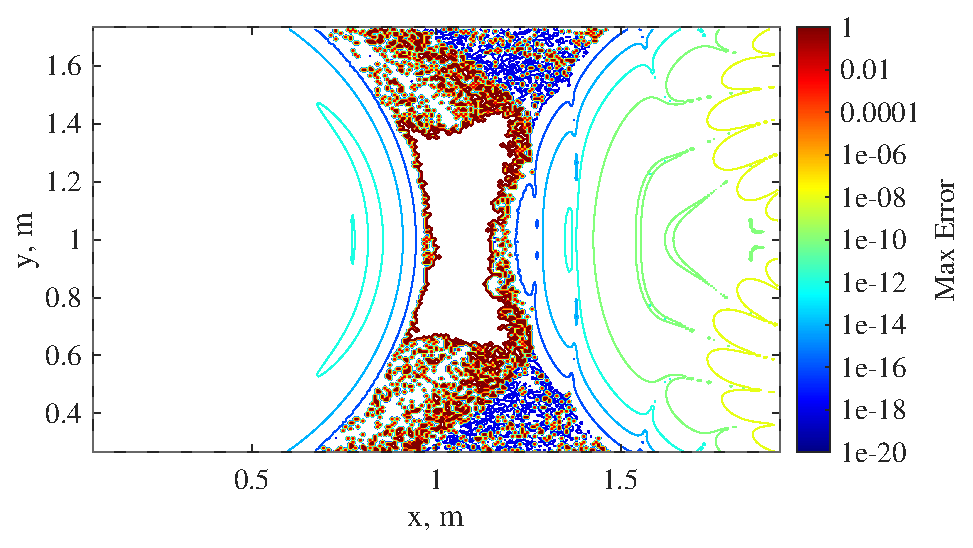
\includegraphics[width=8.5cm]{Figures/TechnicalAchievement/Res/ncErrorDistrAt08s.eps}}
        \caption{}
        \label{fig:ncErrorDistr}
    \end{subfigure}
    \caption{\textbf{(a)} Surface plot of acoustic and entropy waves at $t=0.8 \ \mathrm{s}$ with $D_y=40\Delta x$ and $D_x=10\Delta x$. \textbf{(b)} Distribution of PML-induced error in Euler domain from propagating acoustic and entropy waves.}
    \label{fig:nc}
\end{figure}



